\documentclass[notes,slidesec,a4]{seminar}
\usepackage[spanish]{babel}
\usepackage[utf8]{inputenc}

\usepackage{t-gsyc-6}
\usepackage{fancybox}
\usepackage{graphics}
\usepackage{moreverb}
\usepackage{alltt}
\usepackage{html}
\usepackage{hthtml}
\usepackage{amsmath}
\usepackage[normalsize]{subfigure}
\usepackage{url}
\usepackage{listings}

\usepackage{eurosym}

\title{VisualHFSM 5.0}
\author{Samuel Rey Escudero}

\cop{Samuel Rey Escudero}
\address{samuel.rey.escudero@gmail.com}

\begin{document}
\maketitle

%%--------------------------------------------------------------

\begin{hslide}
\slsect{Índice}
\begin{itemize}
\item Introducción 
\item Objetivos
\item Infraestructura
\item VisualHFSM 5.0
\item Experimentos
\item Conclusiones
\end{itemize}
\end{hslide}

%%--------------------------------------------------------------

\begin{hslide}
\slsect{Introducción}
\begin{itemize}
\item La {\bf inteligencia} de los robots radica en su {\bf software}.
\item Existen diversos métodos para su programación.
\end{itemize}


\begin{minipage}[t]{0.5\textwidth}
\begin{center}
	\begin{itemize}
		\item Programación visual.
	\end{itemize}
	\begin{figure}
		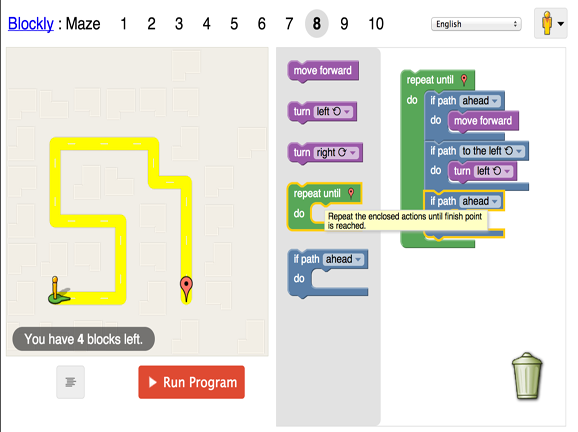
\includegraphics[height=2cm]{imgs/blockly.png}
		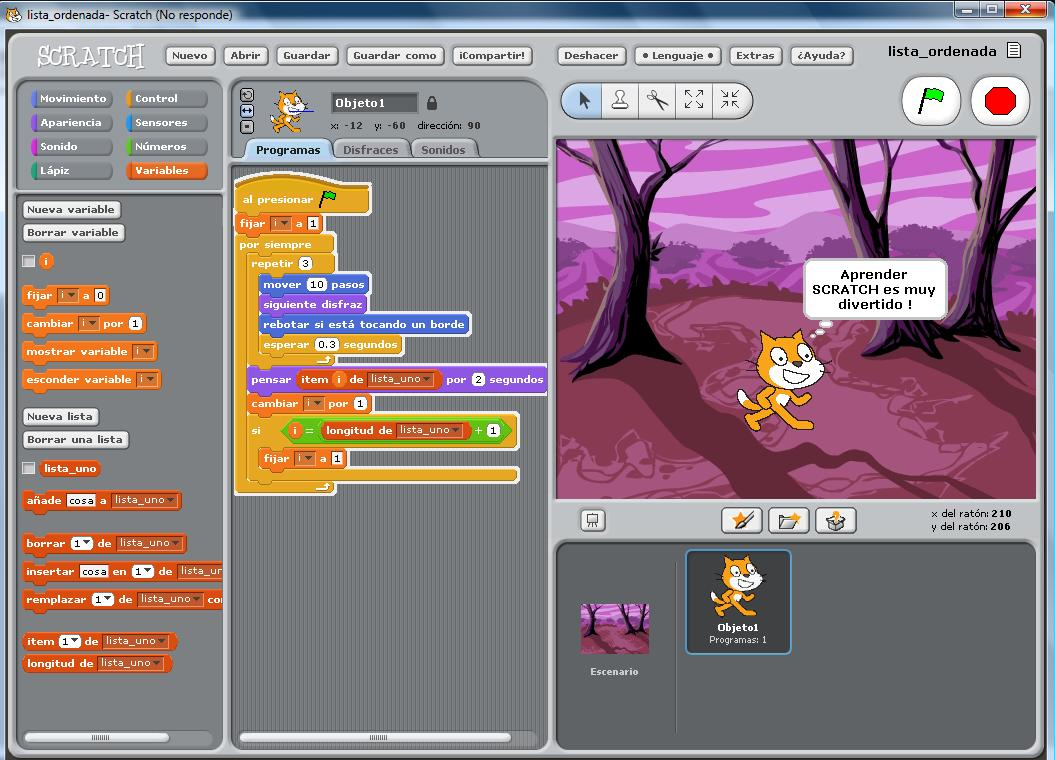
\includegraphics[height=2cm]{imgs/scratch.jpg}
	\end{figure}
\end{center}
\end{minipage} \hfill
\begin{minipage}[t]{0.5\textwidth}
\begin{center}
	\begin{itemize}
		\item Autómatas de estado finito.
	\end{itemize}
	\begin{figure}
		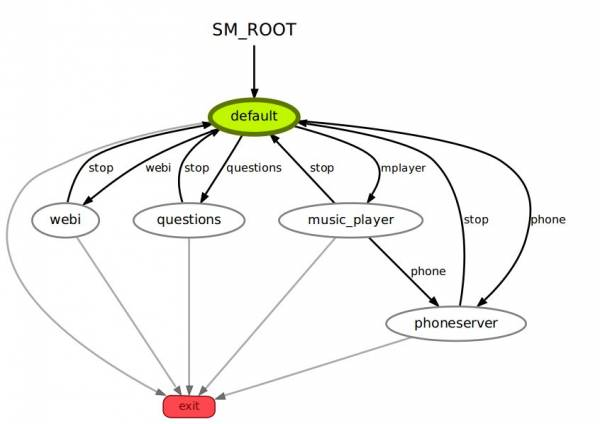
\includegraphics[height=2cm]{imgs/smach.jpg}
		%\hspace{0.6cm}
		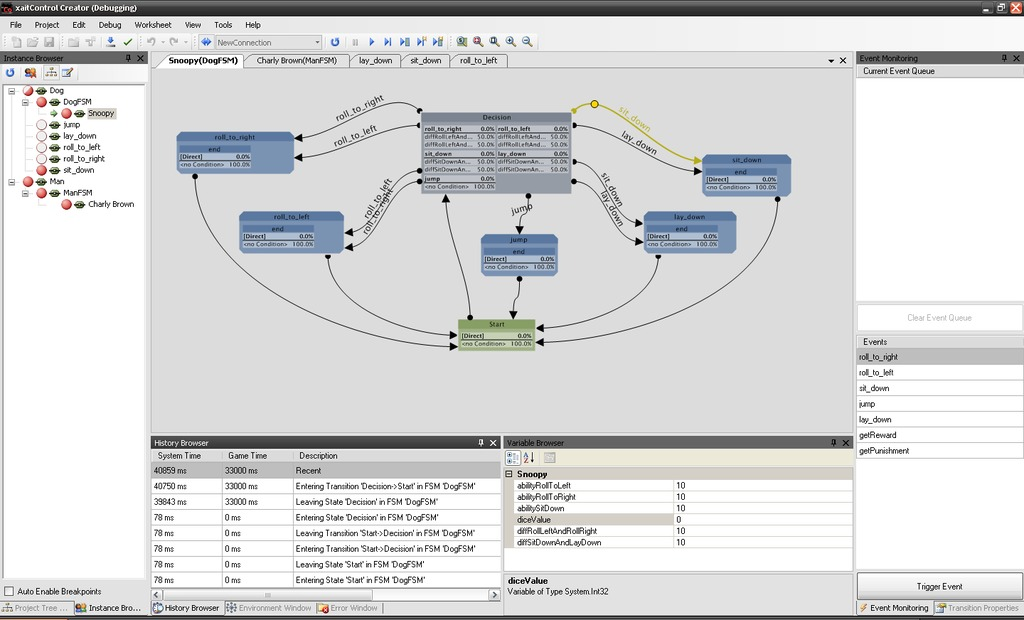
\includegraphics[height=2cm]{imgs/xaitControl.jpg}
	\end{figure}
\end{center}
\end{minipage}

\end{hslide}

%%--------------------------------------------------------------

\begin{hslide}

VisualHFSM ha ido evolucionando con el paso del tiempo.

\begin{minipage}[t]{0.5\textwidth}
\begin{center}
	\begin{figure}
		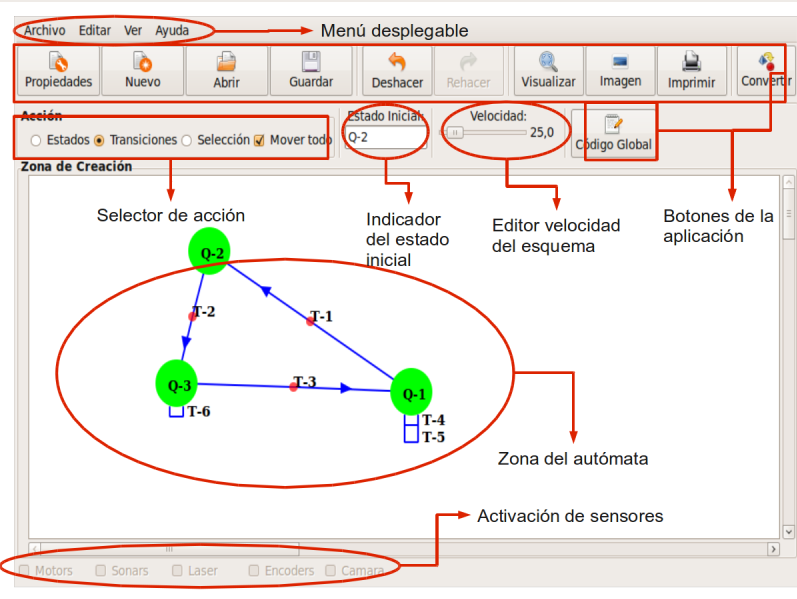
\includegraphics[height=2.5cm]{imgs/visualHFSM1.png}
		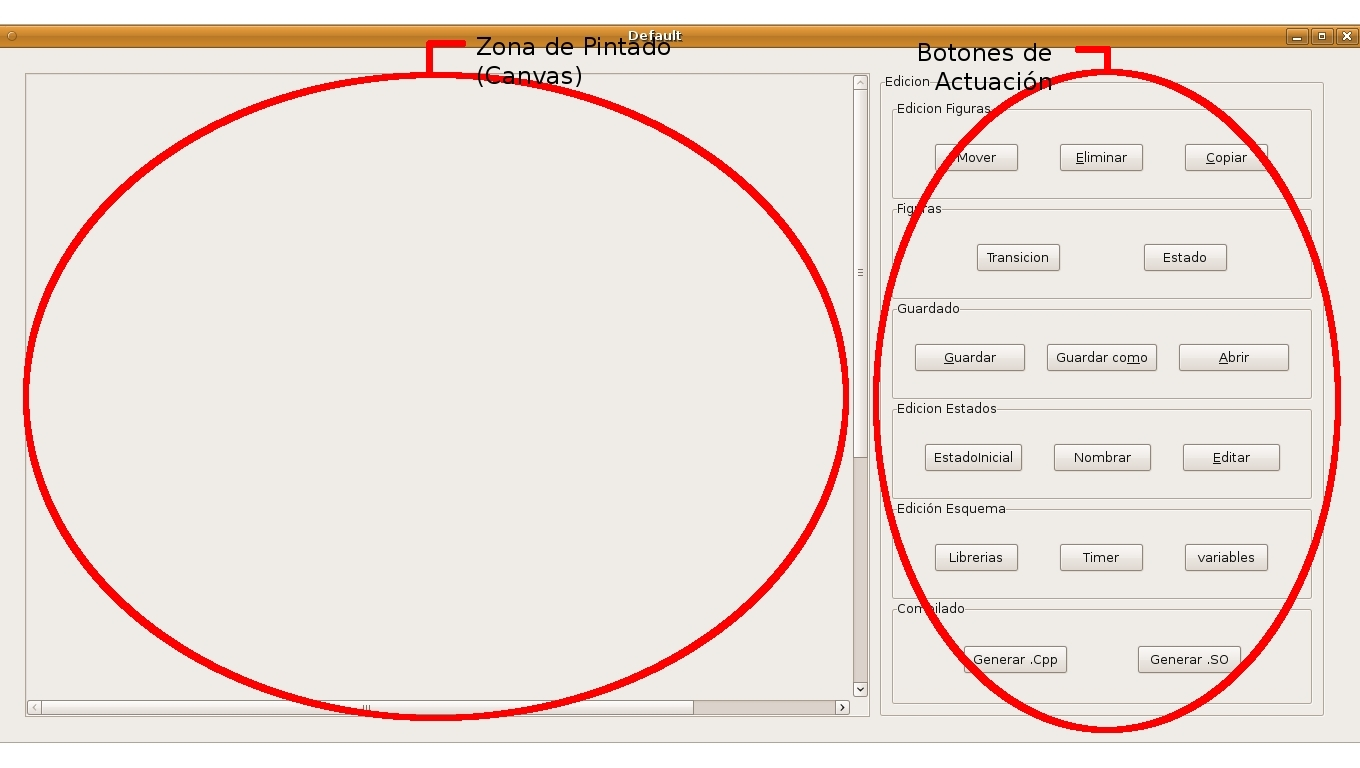
\includegraphics[height=2.5cm]{imgs/visualHFSM2.jpg}
	\end{figure}
\end{center}
\end{minipage} \hfill
\begin{minipage}[t]{0.5\textwidth}
\begin{center}
	\begin{figure}
		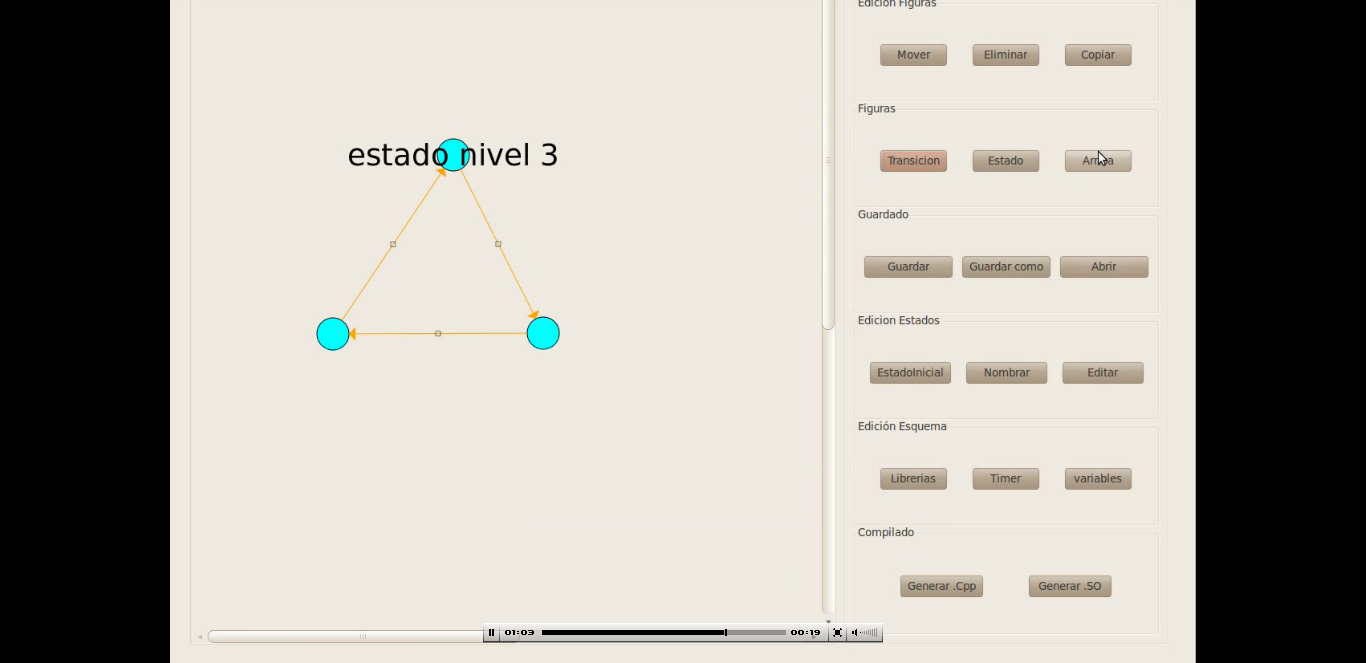
\includegraphics[height=2.5cm]{imgs/visualhfsm3.png}
		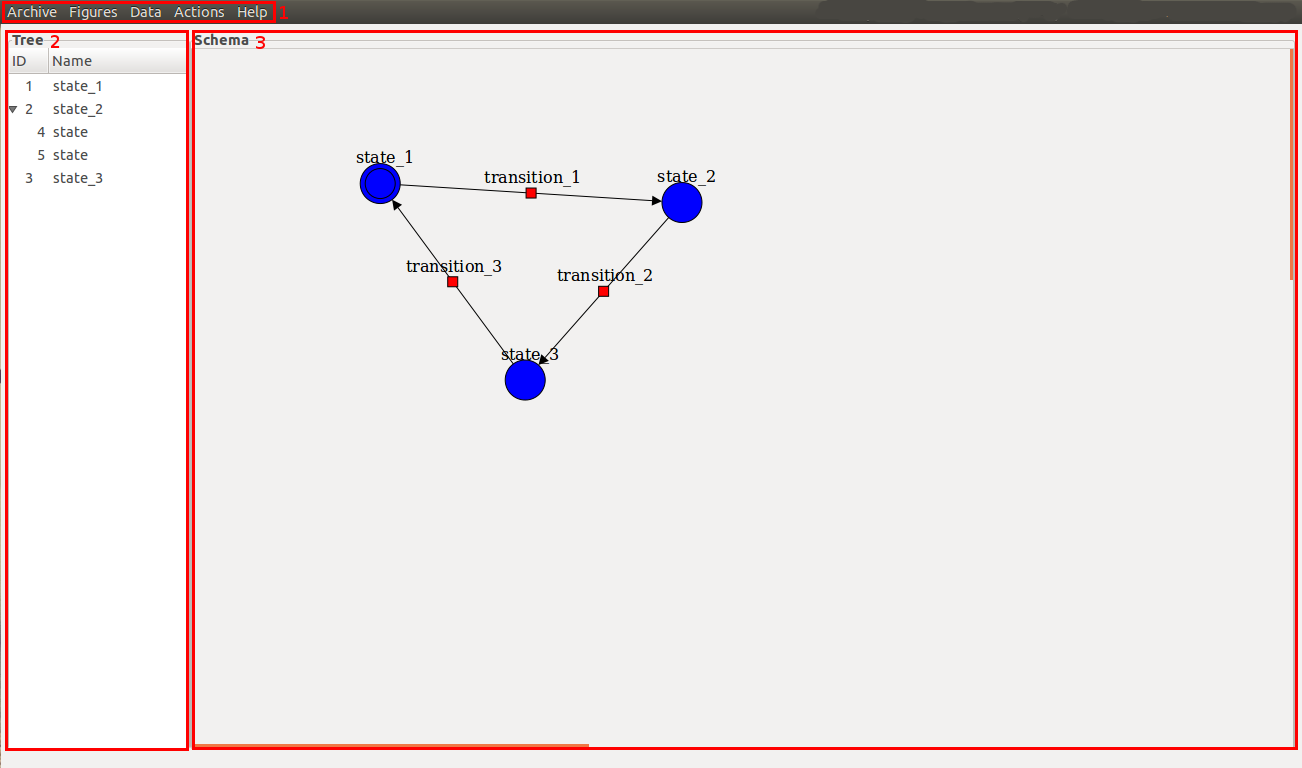
\includegraphics[height=2.5cm]{imgs/visualHFSM4.png}
	\end{figure}
\end{center}
\end{minipage}

\end{hslide}

%%--------------------------------------------------------------

\begin{hslide}
\slsect{Objetivos}

El objetivo principal es alcanzar una versión madura y atractiva de VisualHFSM para que sea utilizada por terceros.

\begin{enumerate}
\item Mejorar la usabilidad y funcionalidad del editor gráfico.
\item Recuperar la GUI en ejecución.
\item Generar componentes en Python.
\item Fomentar la difusión.
\end{enumerate}

\end{hslide}

%%--------------------------------------------------------------

\begin{hslide}

\slsect{Infraestructura}

\begin{minipage}[t]{0.5\textwidth}
\begin{center}
	\begin{itemize}
	\item JdeRobot 5.3.2
	\item Gazebo 5.3
	\item ICE 3.6
	\item GTK+
	\item PyQt4
	\end{itemize}
	\begin{figure}
		
\includegraphics[height=1.5cm]{imgs/logoJdeRobot.png}
	\end{figure}
\end{center}
\end{minipage}
\begin{minipage}[t]{0.5\textwidth}
\begin{center}
	\begin{figure}
		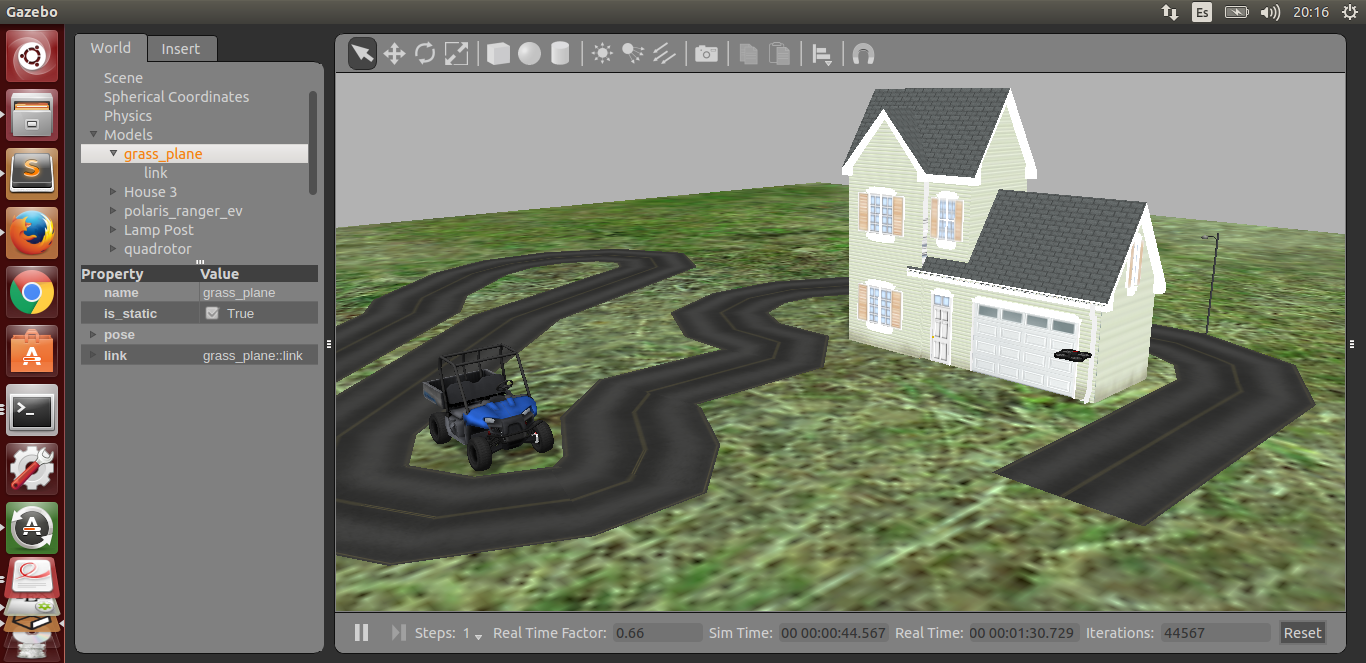
\includegraphics[height=2.3cm]{imgs/gazeboWorld.png}
		\vspace{0.6cm}
		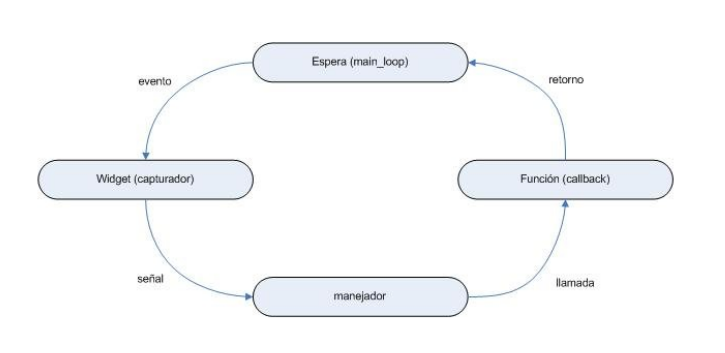
\includegraphics[height=2.3cm]{imgs/bucleGTK.png}
	\end{figure}
\end{center}
\end{minipage}
	
\end{hslide}

%%--------------------------------------------------------------

\begin{hslide}
\slsect{VisualHFSM 5.0}

%%%Con el fin de cumplir os objetivos propuestos, esta versión de VisualHFSM introduce las siguientes novedades:

%\begin{minipage}[t]{0.45\textwidth}
%\begin{center}
\begin{itemize}
\item Mejoras en el editor gráfico.
\item GUI en ejecución para C++.
\item Generación de código en Python.
\item GUI en ejecución para Python.
\item Difusión.
\end{itemize}
%\end{center}
%\end{minipage}
%\begin{minipage}[t]{0.45\textwidth}
\begin{center}
	\begin{figure}
		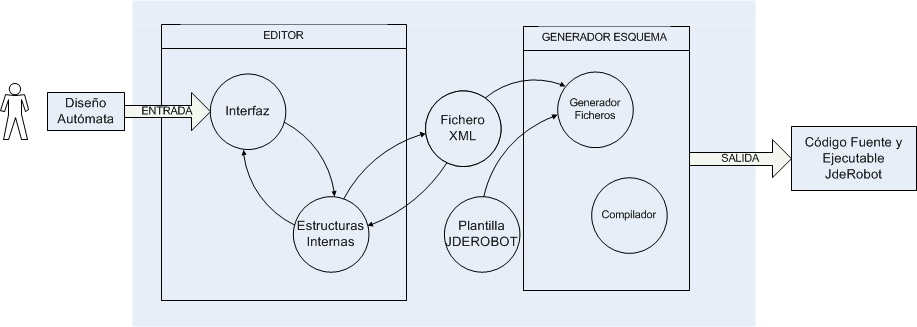
\includegraphics[height=3cm]{imgs/cajaBlanca.jpg}
	\end{figure}
\end{center}
%\end{minipage}

\end{hslide}

%%--------------------------------------------------------------

\begin{hslide}
\slsubsect{Mejoras en el editor gráfico}

\begin{minipage}[t]{0.45\textwidth}
\begin{center}
	\begin{itemize}
	\item Mejor navegación niveles.
	\item Función \texttt{shutDown()} para terminar la ejecución.
	\item Más flexibilidad para crear el archivo de configuración.
	\item Puede ejecutarse desde cualquier directorio.
	%%%\item Corregidos fallos presentes en versiones anteriores.
	\end{itemize}
\end{center}
\end{minipage}\hfill
\begin{minipage}[t]{0.45\textwidth}
\begin{center}
	\begin{figure}
		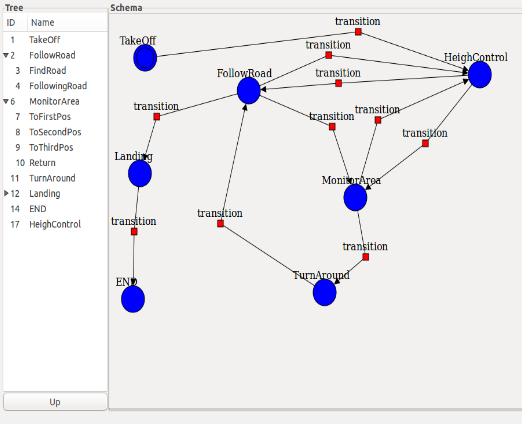
\includegraphics[height=3.5cm]{imgs/editor.png}
		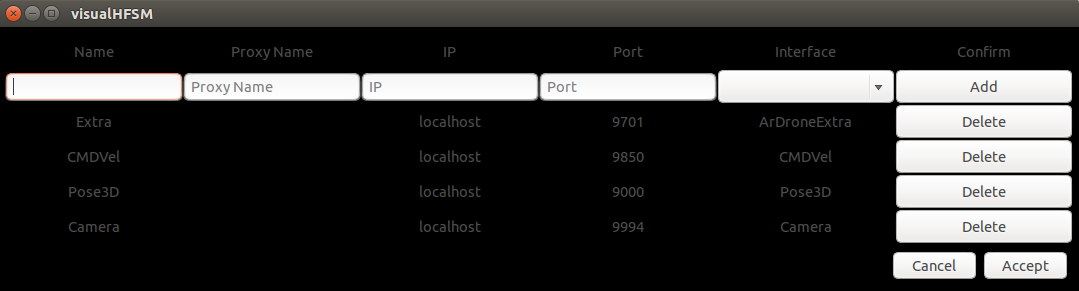
\includegraphics[height=1.5cm]{imgs/configFiles.png}
	\end{figure}
\end{center}
\end{minipage}

\end{hslide}

%%--------------------------------------------------------------

\begin{hslide}
\slsubsect{GUI en ejecución para C++}

\begin{minipage}[t]{0.55\textwidth}
\begin{center}
	\begin{itemize}
	\item Permite observar dinámicamente los estados activos en tiempo de ejecución.
	\item Aspecto similar al editor gráfico.
	\item Desactivada por defecto, se activa con el argumento \textit{--displaygui=true}.
	\item La GUI no depende del XML.
	%\item Se utiliza un objeto \textit{Glib::Dispatcher} para notificar al hilo de la GUI cuando se ha producido un cambio en los estados.
	\item Opción de \textit{autofocus}.
	\end{itemize}
\end{center}
\end{minipage}\hfill
\begin{minipage}[t]{0.4\textwidth}
\begin{center}
	\begin{figure}
		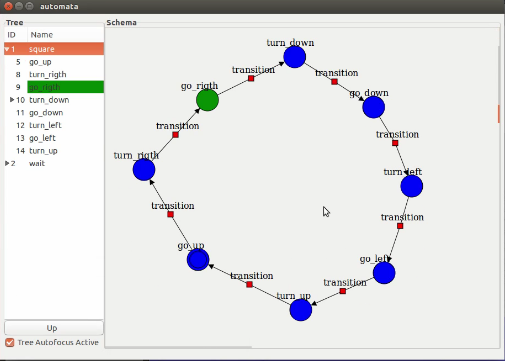
\includegraphics[height=3.5cm]{imgs/newRuntimeGuiCPP.png}
		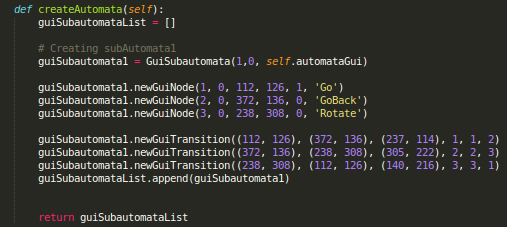
\includegraphics[height=2.3cm]{imgs/createAutomata.png}%Pasarla a transpa con plantilla??
	\end{figure}
\end{center}
\end{minipage}
\end{hslide}

%%--------------------------------------------------------------

\begin{hslide}
\slsubsect{Generación de código Python y su GUI en ejecución.}

\begin{itemize}
\item Da mayor flexibilidad a la herramienta.
\item La plantilla sigue un modelo de OOP.
\item La GUI en ejecución funciona igual que en los componentes de C++.
\item Además permite visualizar más de un nivel a la vez.
\end{itemize}

\begin{center}
	\begin{figure}
		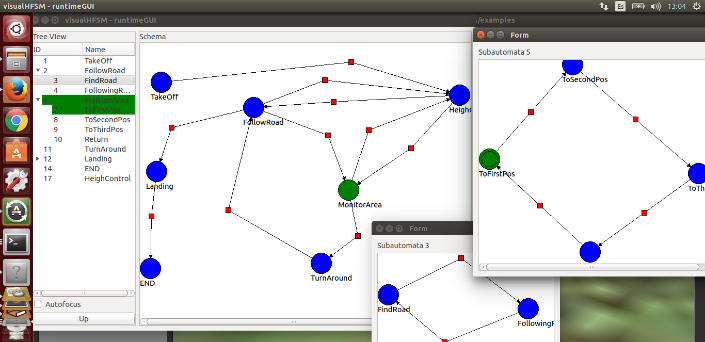
\includegraphics[height=4cm]{imgs/runtime-hierarchy.png}
	\end{figure}
\end{center}

\end{hslide}


%%--------------------------------------------------------------
%Transpa con plantilla python y tal vel la generación en pseudocódigo

\begin{hslide}

\begin{center}
	\begin{figure}
		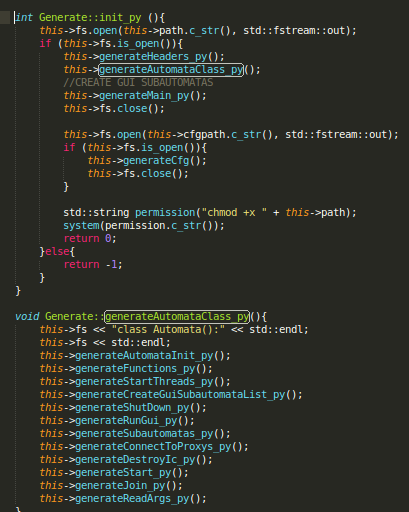
\includegraphics[height=7cm]{imgs/templategenerator.png}
		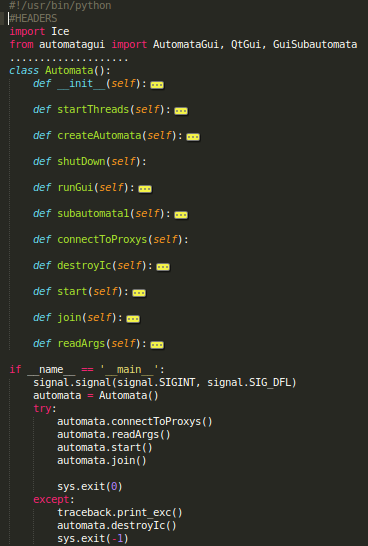
\includegraphics[height=7cm]{imgs/templatecode.png}
	\end{figure}
\end{center}
\end{hslide}

%%--------------------------------------------------------------

\begin{hslide}
\slsubsect{Difusión}

Además de madurar y mejorar la funcionalidad de la herramienta, para que sea utilizada por terceros también nos hemos encargado de:
\begin{itemize}
\item Una documentación web. 
\item Artículo aceptado en el congreso robótico WAF 2016.
\item Práctica Choca-Gira en el entorno docente JdeRobot.
\end{itemize}

\end{hslide}

%%--------------------------------------------------------------

\begin{hslide}
\slsect{Experimentos}

Estos experimentos nos han permitido:

\begin{itemize}
\item Probar que las mejoras añadidas funcionan correctamente.
\item Mostrar la compatibilidad con un nuevo robot: los drones.
\end{itemize}

3 aplicaciones programadas en Python:

\begin{itemize}
\item Choca-Gira.
\item Monitorizar un área.
\item Aplicación Sigue Colores con un drone.
\end{itemize}

\end{hslide}

%%--------------------------------------------------------------

\begin{hslide}
\slsubsect{Choca-Gira}

\begin{itemize}
\item Aplicación sencilla resuelta con un autómata mononivel.
\item Solución a la práctica propuesta en el entorno docente JdeRobot.
\end{itemize}

\begin{center}
\begin{minipage}[t]{0.45\textwidth}
	\begin{figure}
		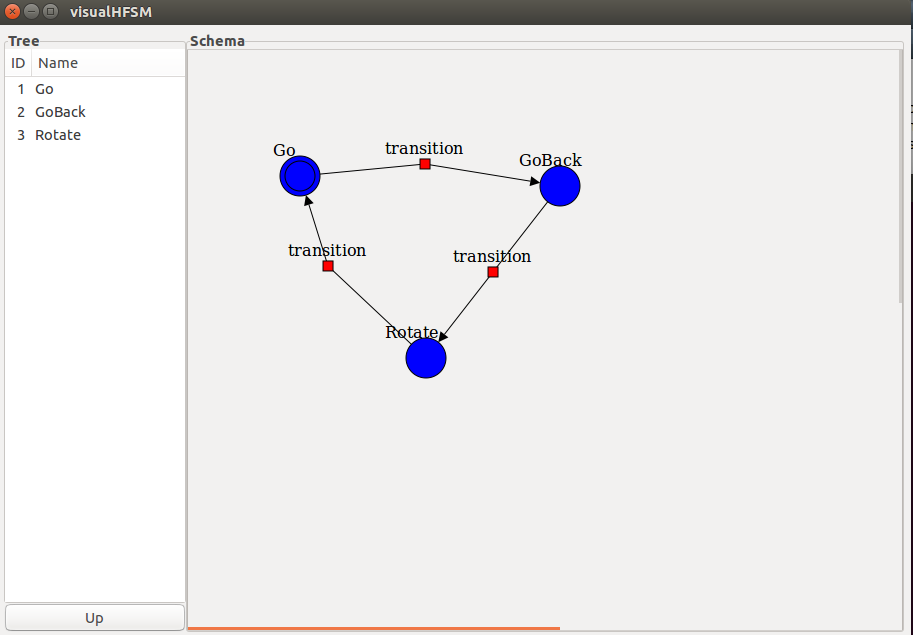
\includegraphics[height=3cm]{imgs/bumpAndGoDiagram.png}
	\end{figure}
\end{minipage}
\begin{minipage}[t]{0.45\textwidth}
	\begin{figure}
		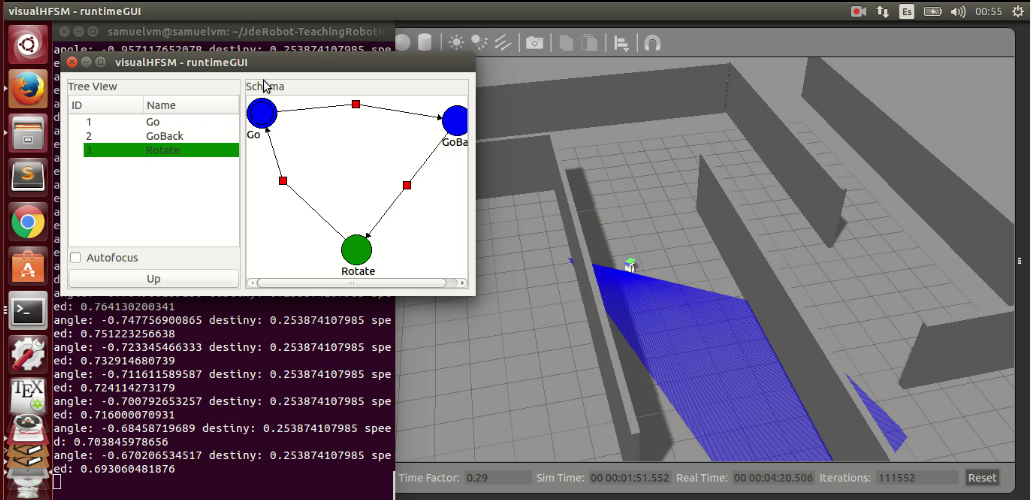
\includegraphics[height=3cm]{imgs/BAGRotate.png}
	\end{figure}
\end{minipage}
\end{center}

\end{hslide}


%%--------------------------------------------------------------

\begin{hslide}
\slsubsect{Monitorizar un área}

\begin{itemize}
\item Comportamiento más complejo.
\item Autómata multinivel.
\item Prueba la compatibilidad de la interfaz del ArDrone en VisualHFSM.
\end{itemize}

\begin{center}
\begin{minipage}[t]{0.45\textwidth}
	\begin{figure}
		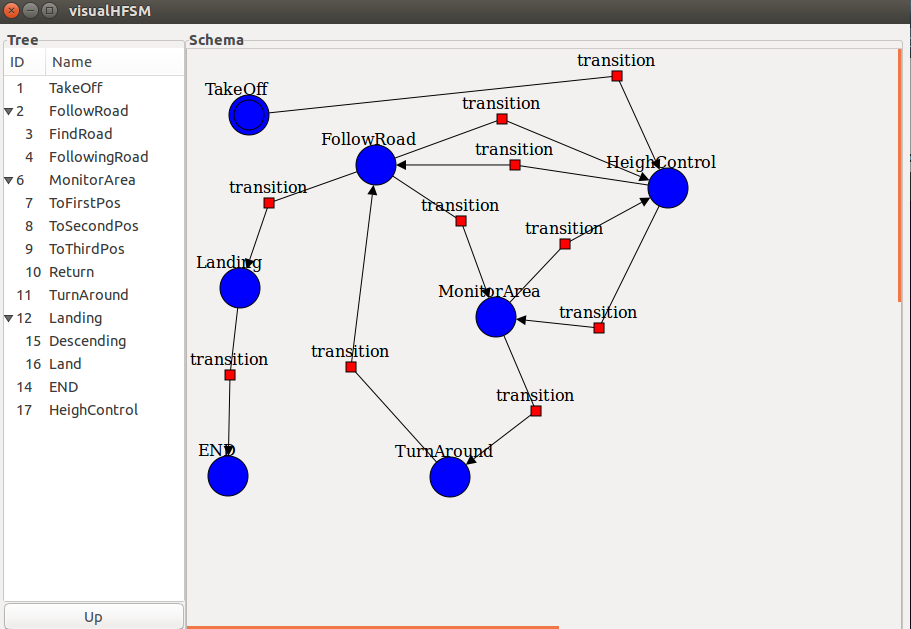
\includegraphics[height=3cm]{imgs/monitorArea.png}
	\end{figure}
\end{minipage}
\begin{minipage}[t]{0.45\textwidth}
	\begin{figure}
		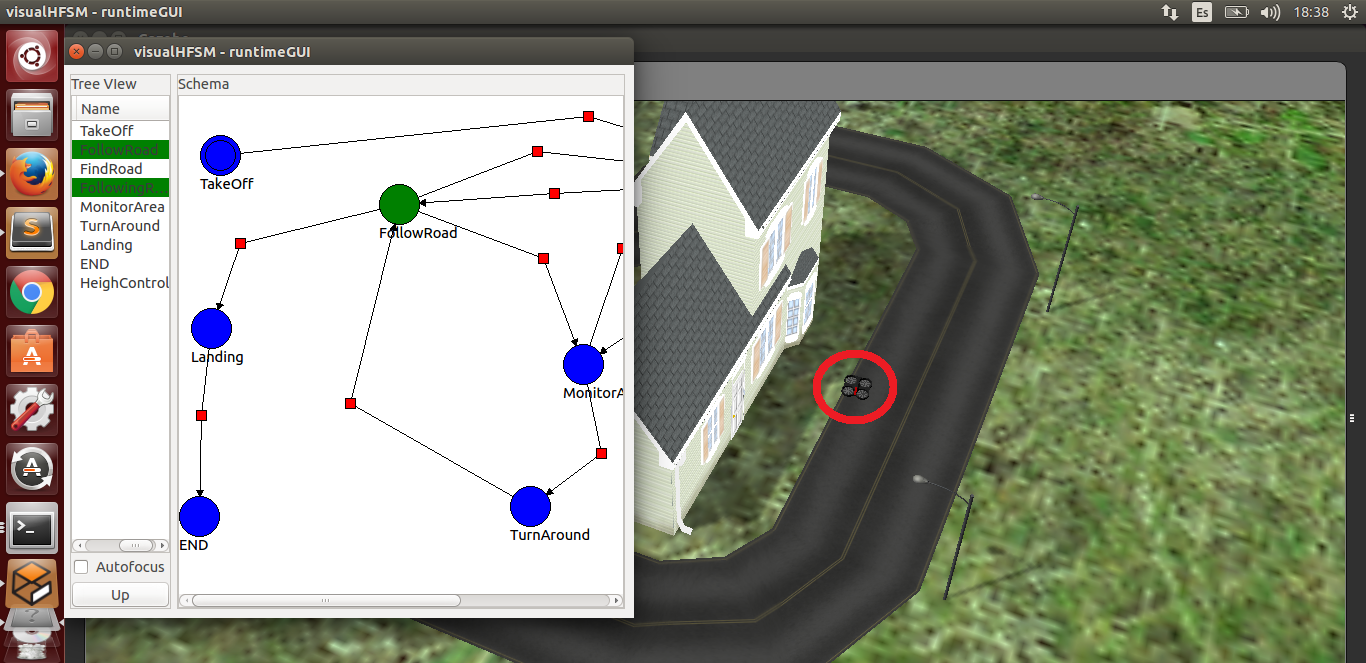
\includegraphics[height=3cm]{imgs/followingRoad.png}
	\end{figure}
\end{minipage}
\end{center}

\end{hslide}


%%--------------------------------------------------------------

\begin{hslide}
\slsubsect{Sigue Colores}

\begin{itemize}
\item Los componentes generados son compatibles con robots reales.
\item Muestra la potencia del autómata frente a sistemas reactivos puros.
\end{itemize}

\begin{center}
\begin{minipage}[t]{0.45\textwidth}
	\begin{figure}
		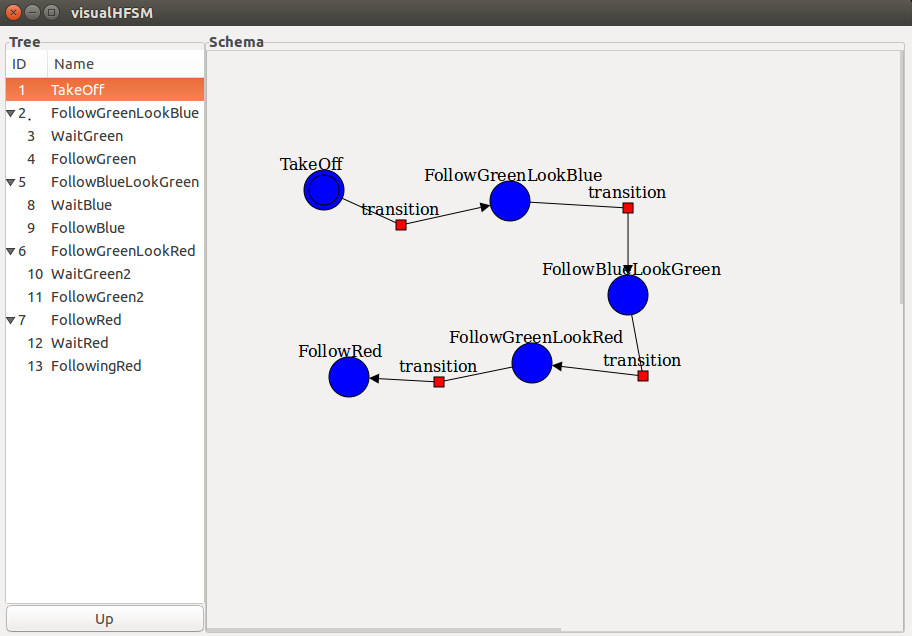
\includegraphics[height=3cm]{imgs/colorsDiagram.png}
	\end{figure}
\end{minipage}
\begin{minipage}[t]{0.45\textwidth}
	\begin{figure}
		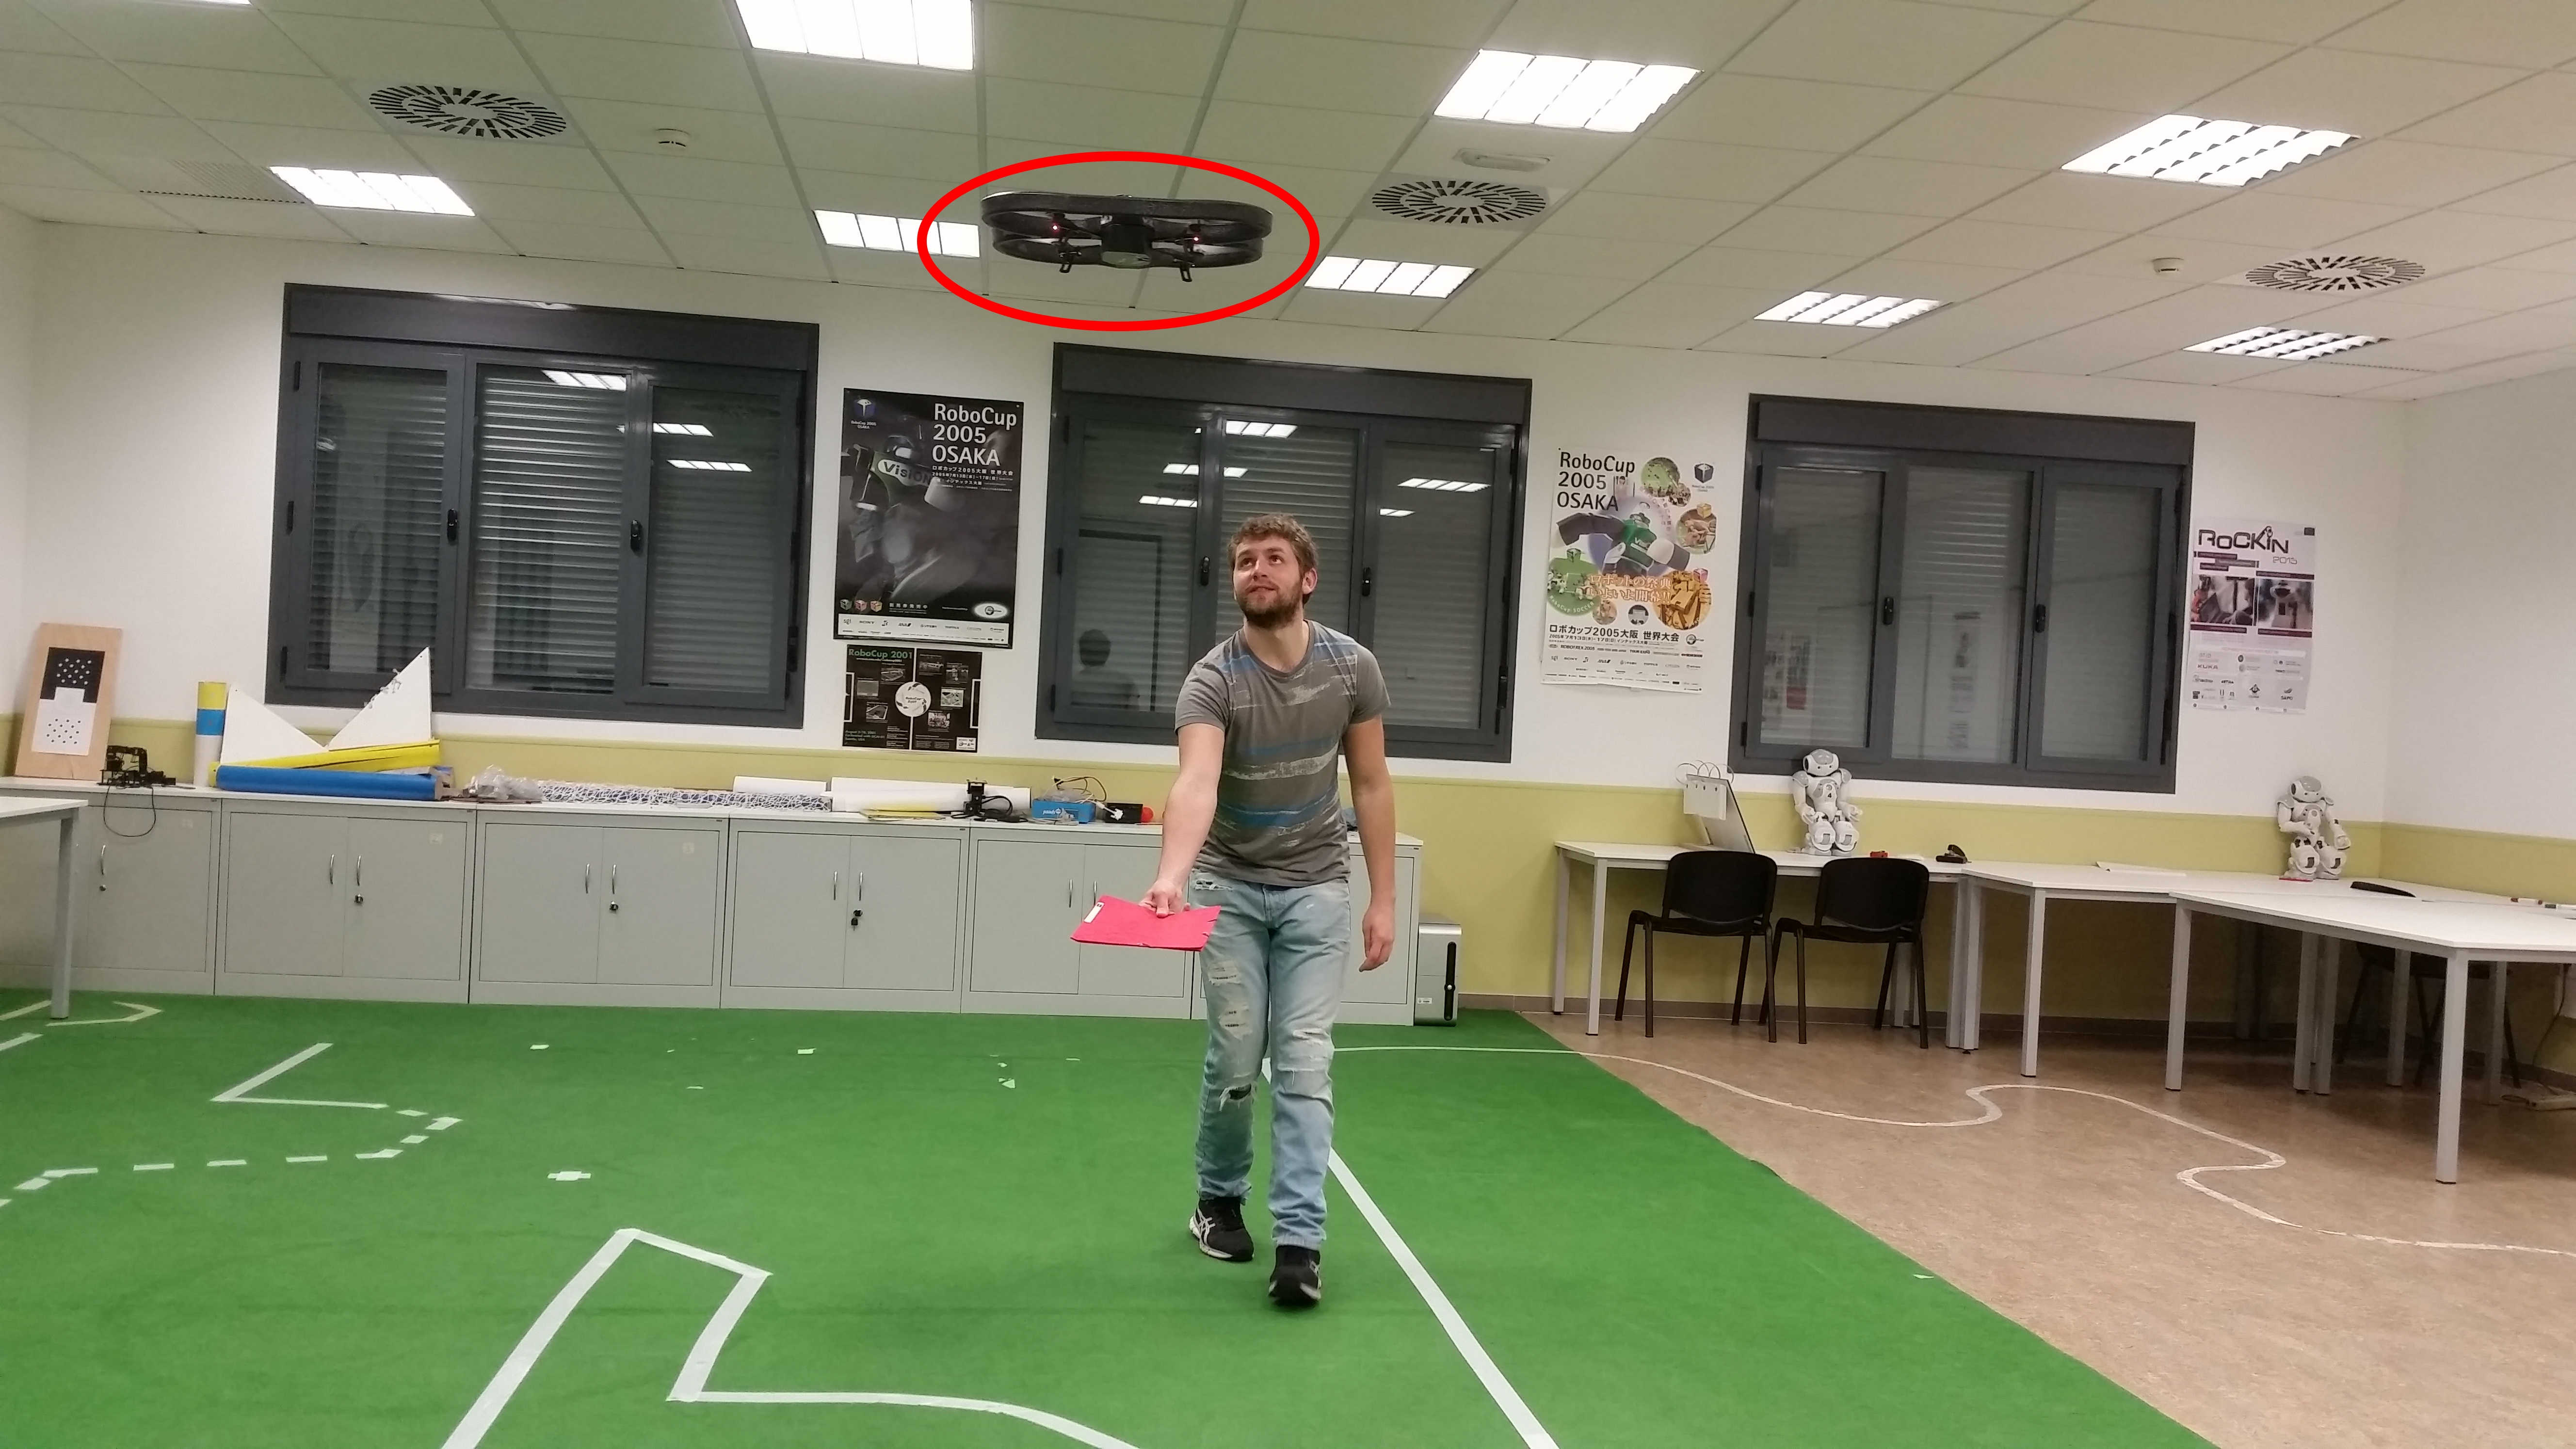
\includegraphics[height=3cm]{imgs/followingRed.jpg}
	\end{figure}
\end{minipage}
\end{center}

\end{hslide}

%%--------------------------------------------------------------

\begin{hslide}
\slsect{Conclusiones y trabajos futuros}

\begin{enumerate}
\item Se ha mejorado la usabilidad y robustez del editor gráfico.
\item Se ha añadido la GUI en tiempo de ejecución con jerarquía para C++.
\item VisualHFSM es capaz de generar componentes en Python.
\item Los componentes en Python disponen de GUI en tiempo de ejecución.
\item Se ha realizado un trabajo de difusión para fomentar su uso.
\end{enumerate}

%%% CÓDIGO!
\textbf{Más de 2500 líneas de código.}
%Sin contar bugs resueltos ni retoques en clases sueltas ni los archivos de las GUIs ni ejemplos



\vspace{1cm}
\begin{itemize}
\item Inspección variables en ejecución.
\item Botón de parada segura en tiempo de ejecución.
%\item Acercar ViualHFSM más a un LPV con fines didácticos.
\end{itemize}

\end{hslide}

\end{document}

